\chapter{Saubere Architektur}
\label{ch:quality/clean-arch}

Hat dein Mod eine ordentliche Größe erreicht, wird es immer schwerer,
den Code sauber und fehlerfrei zu halten. Bei einer dynamisch
typisierten Sprache wie Lua ist das ein besonders großes Problem, denn
der Compiler hilft dir kaum dabei, etwa Typen richtig zu verwenden.

Dieses Kapitel behandelt wichtige Konzepte, die deinen Code sauber
halten, und verbreitete Entwurfsmuster dafür. Es ist nicht als
Vorschrift gemeint, sondern soll dir zeigen, welche Möglichkeiten es
gibt. Den einen richtigen Weg, einen Mod zu entwerfen, gibt es nicht;
was guter Mod-Entwurf ist, ist sehr subjektiv.

\section{Kohäsion, Kopplung und Trennung der
Belange}\label{kohuxe4sion-kopplung-und-trennung-der-belange}

Ohne Planung verkommt ein Programmierprojekt mit der Zeit zu
Spaghetticode. Spaghetticode zeichnet sich durch fehlende Struktur aus
-- aller Code ist zusammengewürfelt, ohne klare Grenzen. Am Ende ist das
Projekt nicht mehr wartbar und wird aufgegeben.

Das Gegenteil ist, dein Projekt als Sammlung kleinerer,
zusammenwirkender Programme oder Codebereiche zu entwerfen.

\begin{quote}
Inside every large program, there is a small program trying to get out.

In jedem großen Programm steckt ein kleines, das herauswill.

--- C. A. R. Hoare
\end{quote}

Dabei solltest du eine \emph{Trennung der Belange} (\emph{separation of
concerns}) erreichen: Jeder Bereich ist klar abgegrenzt und kümmert sich
um eine eigene Aufgabe.

Diese Programme oder Bereiche sollten zwei Eigenschaften haben:

\begin{itemize}
\tightlist
\item
  \textbf{Hohe Kohäsion} -- was in einem Bereich steht, gehört eng
  zusammen.
\item
  \textbf{Geringe Kopplung} -- halte die Abhängigkeiten zwischen
  Bereichen so gering wie möglich und verlass dich nicht auf interne
  Umsetzungen. Geringe Kopplung ist sehr sinnvoll, denn dann lassen sich
  die APIs einzelner Bereiche leichter ändern.
\end{itemize}

Das gilt sowohl für die Beziehungen zwischen Mods als auch für die
Beziehungen zwischen Bereichen innerhalb eines Mods.

\section{Beobachter}\label{beobachter}

Ein einfacher Weg, Codebereiche voneinander zu trennen, ist das
Beobachter-Muster (\emph{Observer}).

Nehmen wir als Beispiel eine Errungenschaft, die freigeschaltet wird,
wenn ein Spieler zum ersten Mal ein seltenes Tier erlegt. Der naive
Ansatz wäre, Errungenschaftscode in die Funktion für den Tod eines Mobs
zu schreiben, die den Mob-Namen prüft und bei Übereinstimmung die
Errungenschaft freischaltet. Das ist aber keine gute Idee, denn damit
ist der Mob-Mod an den Errungenschaftscode gekoppelt. Machst du so
weiter -- fügst etwa auch noch Erfahrungspunkte in den Code für den Tod
eines Mobs ein --, entsteht schnell ein Gewirr von Abhängigkeiten.

Hier kommt das Beobachter-Muster ins Spiel. Statt dass sich der Mod
\texttt{mymobs} um Errungenschaften kümmert, bietet er anderen
Codebereichen die Möglichkeit, ihr Interesse an einem Ereignis
anzumelden und Daten dazu zu erhalten.

\begin{Shaded}
\begin{Highlighting}[]
\VariableTok{mymobs}\OperatorTok{.}\VariableTok{registered\_on\_death} \OperatorTok{=} \OperatorTok{\{\}}
\KeywordTok{function} \VariableTok{mymobs}\OperatorTok{.}\NormalTok{register\_on\_death}\OperatorTok{(}\VariableTok{func}\OperatorTok{)}
    \FunctionTok{table.insert}\OperatorTok{(}\VariableTok{mymobs}\OperatorTok{.}\VariableTok{registered\_on\_death}\OperatorTok{,} \VariableTok{func}\OperatorTok{)}
\KeywordTok{end}

\CommentTok{{-}{-} im Code für den Tod eines Mobs}
\ControlFlowTok{for} \VariableTok{i} \OperatorTok{=} \DecValTok{1}\OperatorTok{,} \OperatorTok{\#}\VariableTok{mymobs}\OperatorTok{.}\VariableTok{registered\_on\_death} \ControlFlowTok{do}
    \VariableTok{mymobs}\OperatorTok{.}\VariableTok{registered\_on\_death}\OperatorTok{[}\VariableTok{i}\OperatorTok{](}\VariableTok{entity}\OperatorTok{,} \VariableTok{reason}\OperatorTok{)}
\ControlFlowTok{end}
\end{Highlighting}
\end{Shaded}

Der andere Code meldet dann sein Interesse an:

\begin{Shaded}
\begin{Highlighting}[]
\VariableTok{mymobs}\OperatorTok{.}\NormalTok{register\_on\_death}\OperatorTok{(}\KeywordTok{function}\OperatorTok{(}\VariableTok{mob}\OperatorTok{,} \VariableTok{reason}\OperatorTok{)}
    \ControlFlowTok{if}
        \VariableTok{reason}\OperatorTok{.}\VariableTok{type} \OperatorTok{==} \StringTok{"punch"}
        \KeywordTok{and} \VariableTok{reason}\OperatorTok{.}\VariableTok{object}
        \KeywordTok{and} \VariableTok{reason}\OperatorTok{.}\VariableTok{object}\OperatorTok{:}\NormalTok{is\_player}\OperatorTok{()}
    \ControlFlowTok{then}
        \VariableTok{awards}\OperatorTok{.}\NormalTok{notify\_mob\_kill}\OperatorTok{(}\VariableTok{reason}\OperatorTok{.}\VariableTok{object}\OperatorTok{,} \VariableTok{mob}\OperatorTok{.}\VariableTok{name}\OperatorTok{)}
    \ControlFlowTok{end}
\KeywordTok{end}\OperatorTok{)}
\end{Highlighting}
\end{Shaded}

Vielleicht denkst du jetzt: Moment, das kommt mir bekannt vor. Richtig!
Die Luanti-API baut stark auf dem Beobachter-Muster auf, damit sich die
Engine nicht darum kümmern muss, wer auf etwas wartet.

\section{Model-View-Controller}\label{model-view-controller}

Im nächsten Kapitel geht es darum, deinen Code automatisch zu testen.
Eine Schwierigkeit dabei ist, die Logik (Berechnungen, was getan werden
soll) möglichst weit von API-Aufrufen (\texttt{core.\allowbreak{}*},
andere Mods) zu trennen.

Ein Weg dahin ist, dir Folgendes zu überlegen:

\begin{itemize}
\tightlist
\item
  Welche \textbf{Daten} hast du?
\item
  Welche \textbf{Aktionen} kannst du mit diesen Daten ausführen?
\item
  Wie lösen \textbf{Ereignisse} (etwa Formspecs\index{formspec@Formspec}
  oder Schläge) diese Aktionen aus, und wie bewirken die Aktionen etwas
  in der Engine?
\end{itemize}

Nehmen wir einen Mod zum Schutz von Grundstücken. Die Daten sind die
Grundstücke und die zugehörigen Metadaten.\index{metadaten@Metadaten}
Die Aktionen sind \texttt{create}, \texttt{edit} und \texttt{delete}.
Ausgelöst werden sie durch Chatbefehle\index{chatbefehl@Chatbefehl} und
Formspec-Eingaben. Diese drei Bereiche lassen sich meist gut voneinander
trennen.

In deinen Tests kannst du dann sicherstellen, dass eine ausgelöste
Aktion das Richtige mit den Daten macht. Dass ein Ereignis eine Aktion
auslöst, musst du nicht testen -- dafür bräuchtest du die Luanti-API,
und dieser Codebereich sollte ohnehin so klein wie möglich sein.

Die Datenschicht schreibst du in reinem Lua. „Rein`` heißt hier, dass
die Funktionen auch außerhalb von Luanti laufen könnten -- keine
Funktion der Engine wird aufgerufen.

\begin{Shaded}
\begin{Highlighting}[]
\CommentTok{{-}{-} Daten}
\KeywordTok{function} \VariableTok{land}\OperatorTok{.}\NormalTok{create}\OperatorTok{(}\VariableTok{name}\OperatorTok{,} \VariableTok{area\_name}\OperatorTok{)}
    \VariableTok{land}\OperatorTok{.}\VariableTok{lands}\OperatorTok{[}\VariableTok{area\_name}\OperatorTok{]} \OperatorTok{=} \OperatorTok{\{}
        \VariableTok{name} \OperatorTok{=} \VariableTok{area\_name}\OperatorTok{,}
        \VariableTok{owner} \OperatorTok{=} \VariableTok{name}\OperatorTok{,}
        \CommentTok{{-}{-} weitere Angaben}
    \OperatorTok{\}}
\KeywordTok{end}

\KeywordTok{function} \VariableTok{land}\OperatorTok{.}\NormalTok{get\_by\_name}\OperatorTok{(}\VariableTok{area\_name}\OperatorTok{)}
    \ControlFlowTok{return} \VariableTok{land}\OperatorTok{.}\VariableTok{lands}\OperatorTok{[}\VariableTok{area\_name}\OperatorTok{]}
\KeywordTok{end}
\end{Highlighting}
\end{Shaded}

Auch die Aktionen sollten rein sein, wobei Aufrufe anderer Funktionen
hier eher vertretbar sind als oben.

\begin{Shaded}
\begin{Highlighting}[]
\CommentTok{{-}{-} Controller}
\KeywordTok{function} \VariableTok{land}\OperatorTok{.}\NormalTok{handle\_create\_submit}\OperatorTok{(}\VariableTok{name}\OperatorTok{,} \VariableTok{area\_name}\OperatorTok{)}
    \CommentTok{{-}{-} Verarbeitung (etwa Überschneidungen,}
    \CommentTok{{-}{-} Kontingente und Rechte prüfen)}

    \VariableTok{land}\OperatorTok{.}\NormalTok{create}\OperatorTok{(}\VariableTok{name}\OperatorTok{,} \VariableTok{area\_name}\OperatorTok{)}
\KeywordTok{end}

\KeywordTok{function} \VariableTok{land}\OperatorTok{.}\NormalTok{handle\_creation\_request}\OperatorTok{(}\VariableTok{name}\OperatorTok{)}
    \CommentTok{{-}{-} Ein schlechtes Beispiel, wie später erklärt}
    \VariableTok{land}\OperatorTok{.}\NormalTok{show\_create\_formspec}\OperatorTok{(}\VariableTok{name}\OperatorTok{)}
\KeywordTok{end}
\end{Highlighting}
\end{Shaded}

Die Ereignis-Handler müssen mit der Luanti-API arbeiten. Halte die
Berechnungen hier so gering wie möglich, denn diesen Bereich kannst du
nur schwer testen.

\begin{Shaded}
\begin{Highlighting}[]
\CommentTok{{-}{-} View}
\KeywordTok{function} \VariableTok{land}\OperatorTok{.}\NormalTok{show\_create\_formspec}\OperatorTok{(}\VariableTok{name}\OperatorTok{)}
    \CommentTok{{-}{-} Hier gibt es keine komplexen Berechnungen!}
    \VariableTok{core}\OperatorTok{.}\NormalTok{show\_formspec}\OperatorTok{(}
        \VariableTok{name}\OperatorTok{,}
        \StringTok{"land:create"}\OperatorTok{,}
        \VerbatimStringTok{[[}
\VerbatimStringTok{        size[4,3]}
\VerbatimStringTok{        label[1,0;Das ist ein Beispiel]}
\VerbatimStringTok{        field[0,1;3,1;area\_name;]}
\VerbatimStringTok{        button\_exit[0,2;1,1;exit;Beenden]}
\VerbatimStringTok{    ]]}
    \OperatorTok{)}
\KeywordTok{end}

\VariableTok{core}\OperatorTok{.}\NormalTok{register\_chatcommand}\OperatorTok{(}\StringTok{"land"}\OperatorTok{,} \OperatorTok{\{}
    \VariableTok{privs} \OperatorTok{=} \OperatorTok{\{} \VariableTok{land} \OperatorTok{=} \KeywordTok{true} \OperatorTok{\},}
    \VariableTok{func} \OperatorTok{=} \KeywordTok{function}\OperatorTok{(}\VariableTok{name}\OperatorTok{)}
        \VariableTok{land}\OperatorTok{.}\NormalTok{handle\_creation\_request}\OperatorTok{(}\VariableTok{name}\OperatorTok{)}
    \KeywordTok{end}\OperatorTok{,}
\OperatorTok{\})}

\VariableTok{core}\OperatorTok{.}\NormalTok{register\_on\_player\_receive\_fields}\OperatorTok{(}
    \KeywordTok{function}\OperatorTok{(}\VariableTok{player}\OperatorTok{,} \VariableTok{formname}\OperatorTok{,} \VariableTok{fields}\OperatorTok{)}
        \ControlFlowTok{if} \VariableTok{formname} \OperatorTok{\textasciitilde{}=} \StringTok{"land:create"} \ControlFlowTok{then}
            \ControlFlowTok{return}
        \ControlFlowTok{end}
        \VariableTok{land}\OperatorTok{.}\NormalTok{handle\_create\_submit}\OperatorTok{(}
            \VariableTok{player}\OperatorTok{:}\NormalTok{get\_player\_name}\OperatorTok{(),}
            \VariableTok{fields}\OperatorTok{.}\VariableTok{area\_name}
        \OperatorTok{)}
    \KeywordTok{end}
\OperatorTok{)}
\end{Highlighting}
\end{Shaded}

Das ist das Model-View-Controller-Muster. Das \emph{Model} ist eine
Sammlung von Daten mit möglichst wenigen Funktionen. Die \emph{View} ist
eine Sammlung von Funktionen, die auf Ereignisse warten und sie an den
Controller weitergeben; außerdem nimmt sie Aufrufe des Controllers
entgegen, um etwas mit der Luanti-API zu tun. Im \emph{Controller}
fallen die Entscheidungen, und hier finden die meisten Berechnungen
statt.

Der Controller sollte nichts über die Luanti-API wissen -- beachte, dass
es dort keine Luanti-Aufrufe gibt und auch keine View-Funktionen, die
ihnen ähneln. Eine Funktion wie
\texttt{view.\allowbreak{}hud\_\allowbreak{}add(player, def)} sollte es
\emph{nicht} geben. Stattdessen legt die View Aktionen fest, die der
Controller bei ihr anstoßen kann, etwa
\texttt{view.\allowbreak{}add\_\allowbreak{}hud(info)}, wobei
\texttt{info} ein Wert oder eine Tabelle ist, die nichts mit der
Luanti-API zu tun hat.

\begin{figure}
\centering
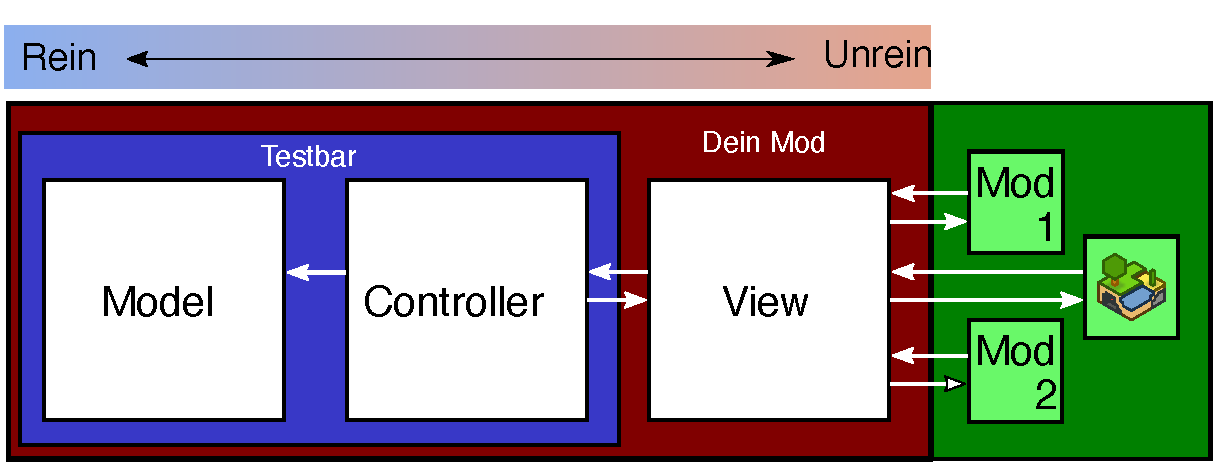
\includegraphics[width=12cm,height=\textheight,keepaspectratio,alt={Model, View und Controller und ihre Verbindungen}]{bilder/mvc_diagram.pdf}
\caption{Model, View und Controller und ihre Verbindungen}
\end{figure}

Wichtig ist, dass jeder Bereich nur mit seinen direkten Nachbarn
kommuniziert, wie im Diagramm gezeigt. So musst du weniger ändern, wenn
du das Innere oder die Schnittstelle eines Bereichs änderst. Um die
Formspec zu ändern, musst du zum Beispiel nur die View anpassen. Um die
API der View zu ändern, musst du nur View und Controller anpassen, das
Model aber gar nicht.

In der Praxis wird dieser Entwurf selten verwendet, weil er die
Komplexität erhöht und den meisten Mods nicht viel bringt. Häufiger
sieht man einen weniger formalen und strengen Entwurf -- Varianten von
API-View.

\subsection{API-View}\label{api-view}

In einer idealen Welt wären die drei Bereiche oben sauber getrennt, und
alle Ereignisse gingen erst durch den Controller, bevor sie zur View
zurückkehren. Die Welt ist aber nicht ideal. Ein guter Kompromiss ist,
den Mod in zwei Teile zu gliedern:

\begin{itemize}
\tightlist
\item
  \textbf{API} -- Das waren oben Model und Controller. Hier sollte
  \texttt{core.\allowbreak{}} nirgends vorkommen.
\item
  \textbf{View} -- Das war auch oben die View. Am besten teilst du sie
  in eigene Dateien für jede Art von Ereignis auf.
\end{itemize}

rubenwardys crafting-Mod\footnote{\url{https://github.com/rubenwardy/crafting}}
folgt ungefähr diesem Entwurf. \texttt{api.\allowbreak{}lua} besteht
fast nur aus reinen Lua-Funktionen für die Datenhaltung und Berechnungen
im Stil eines Controllers. \texttt{gui.\allowbreak{}lua} ist die View
für Formspecs und deren Eingaben, und
\texttt{async\_\allowbreak{}crafter.\allowbreak{}lua} ist View und
Controller für eine Node-Formspec und
Node-Timer.\index{node-timer@Node-Timer}

So aufgeteilt, lässt sich der API-Teil sehr einfach testen, weil er
keine Luanti-APIs verwendet -- wie im nächsten
Kapitel~(Kapitel~\ref{ch:quality/unit-testing}) gezeigt und im
crafting-Mod zu sehen.

\section{Fazit}\label{fazit}

Guter Code-Entwurf ist subjektiv und hängt stark vom jeweiligen Projekt
ab. Als Faustregel gilt: Halte die Kohäsion hoch und die Kopplung
gering. Anders gesagt: Halte zusammen, was zusammengehört, trenne, was
nicht zusammengehört, und halte die Abhängigkeiten einfach.

Sehr zu empfehlen ist das Buch Game Programming Patterns\footnote{\url{http://gameprogrammingpatterns.com/}}
(englisch). Es ist kostenlos online lesbar\footnote{\url{http://gameprogrammingpatterns.com/contents.html}}
und geht viel ausführlicher auf verbreitete Programmiermuster für Spiele
ein.
